%%%%%%%%%%%%%%%%%%%%%%%%%%%%%%%%%%%%%%%%%
% Masters/Doctoral Thesis 
% LaTeX Template
% Version 2.5 (27/8/17)
%
% This template was downloaded from:
% http://www.LaTeXTemplates.com
%
% Version 2.x major modifications by:
% Vel (vel@latextemplates.com)
%
% This template is based on a template by:
% Steve Gunn (http://users.ecs.soton.ac.uk/srg/softwaretools/document/templates/)
% Sunil Patel (http://www.sunilpatel.co.uk/thesis-template/)
%
% Template license:
% CC BY-NC-SA 3.0 (http://creativecommons.org/licenses/by-nc-sa/3.0/)
%
%%%%%%%%%%%%%%%%%%%%%%%%%%%%%%%%%%%%%%%%%

%----------------------------------------------------------------------------------------
%	PACKAGES AND OTHER DOCUMENT CONFIGURATIONS
%----------------------------------------------------------------------------------------

\documentclass[
11pt, % The default document font size, options: 10pt, 11pt, 12pt
oneside, % Two side (alternating margins) for binding by default, uncomment to switch to one side
english,
spanish, % ngerman for German
singlespacing, % Single line spacing, alternatives: onehalfspacing or doublespacing
%draft, % Uncomment to enable draft mode (no pictures, no links, overfull hboxes indicated)
%nolistspacing, % If the document is onehalfspacing or doublespacing, uncomment this to set spacing in lists to single
%liststotoc, % Uncomment to add the list of figures/tables/etc to the table of contents
%toctotoc, % Uncomment to add the main table of contents to the table of contents
parskip, % Uncomment to add space between paragraphs
%nohyperref, % Uncomment to not load the hyperref package
headsepline, % Uncomment to get a line under the header
%chapterinoneline, % Uncomment to place the chapter title next to the number on one line
%consistentlayout, % Uncomment to change the layout of the declaration, abstract and acknowledgements pages to match the default layout
]{MastersDoctoralThesis} % The class file specifying the document structure

%\usepackage[english,spanish]{babel}
\usepackage[utf8]{inputenc} % Required for inputting international characters
\usepackage[T1]{fontenc} % Output font encoding for international characters

\usepackage{mathpazo} % Use the Palatino font by default

%\usepackage{float}

\usepackage[backend=bibtex,style=authoryear,natbib=true]{biblatex} % Use the bibtex backend with the authoryear citation style (which resembles APA)

%\addbibresource{example.bib} % The filename of the bibliography

\usepackage[autostyle=true]{csquotes} % Required to generate language-dependent quotes in the bibliography

%\usepackage{hyperref}

%--------------------------------------------
% Listing for JavaScript
%--------------------------------------------

\usepackage{listings}
\usepackage{color}
\definecolor{antiflash-white}{rgb}{0.95, 0.95, 0.96}
\definecolor{darkgray}{rgb}{.4,.4,.4}
\definecolor{purple}{rgb}{0.65, 0.12, 0.82}

\lstdefinelanguage{JavaScript}{
  keywords={typeof, new, true, false, catch, function, return, null, catch, switch, var, if, in, while, do, else, case, break, extends},
  keywordstyle=\color{blue}\bfseries,
  ndkeywords={class, export, boolean, throw, implements, import, this},
  ndkeywordstyle=\color{darkgray}\bfseries,
  identifierstyle=\color{black},
  sensitive=false,
  comment=[l]{//},
  morecomment=[s]{/*}{*/},
  commentstyle=\color{purple}\ttfamily,
  stringstyle=\color{red}\ttfamily,
  morestring=[b]',
  morestring=[b]"
}


\lstset{
   language=JavaScript,
   backgroundcolor=\color{antiflash-white},
   extendedchars=true,
   basicstyle=\footnotesize\ttfamily,
   showstringspaces=false,
   showspaces=false,
   numbers=left,
   numberstyle=\footnotesize,
   numbersep=10pt,
   tabsize=2,
   breaklines=true,
   showtabs=false,
   captionpos=b,
	 frame=top,
	 frame=bottom
}




%----------------------------------------------------------------------------------------
%	MARGIN SETTINGS
%----------------------------------------------------------------------------------------

\geometry{
	paper=a4paper, % Change to letterpaper for US letter
	inner=2.5cm, % Inner margin
	outer=3.8cm, % Outer margin
	bindingoffset=.5cm, % Binding offset
	top=1.5cm, % Top margin
	bottom=1.5cm, % Bottom margin
	%showframe, % Uncomment to show how the type block is set on the page
}

%----------------------------------------------------------------------------------------
%	THESIS INFORMATION
%----------------------------------------------------------------------------------------

\thesistitle{Thesis Title} % Your thesis title, this is used in the title and abstract, print it elsewhere with \ttitle
\supervisor{Dr. James \textsc{Smith}} % Your supervisor's name, this is used in the title page, print it elsewhere with \supname
\examiner{} % Your examiner's name, this is not currently used anywhere in the template, print it elsewhere with \examname
\degree{} % Your degree name, this is used in the title page and abstract, print it elsewhere with \degreename
\author{Ricardo \textsc{Ferro Moreno}} % Your name, this is used in the title page and abstract, print it elsewhere with \authorname
\addresses{} % Your address, this is not currently used anywhere in the template, print it elsewhere with \addressname

\subject{Biological Sciences} % Your subject area, this is not currently used anywhere in the template, print it elsewhere with \subjectname
\keywords{} % Keywords for your thesis, this is not currently used anywhere in the template, print it elsewhere with \keywordnames
\university{\href{http://www.uns.edu.ar}{Universidad Nacional del Sur}} % Your university's name and URL, this is used in the title page and abstract, print it elsewhere with \univname
\department{\href{http://cs.uns.edu.ar}{Departamento de Ciencias e Ingeniería de la Computación}} % Your department's name and URL, this is used in the title page and abstract, print it elsewhere with \deptname
\group{\href{http://cs.uns.edu.ar}{UNS}} % Your research group's name and URL, this is used in the title page, print it elsewhere with \groupname
\faculty{\href{http://cs.uns.edu.ar}{UNS}} % Your faculty's name and URL, this is used in the title page and abstract, print it elsewhere with \facname

\AtBeginDocument{
\hypersetup{pdftitle=\ttitle} % Set the PDF's title to your title
\hypersetup{pdfauthor=\authorname} % Set the PDF's author to your name
\hypersetup{pdfkeywords=\keywordnames} % Set the PDF's keywords to your keywords
}

\begin{document}

\frontmatter % Use roman page numbering style (i, ii, iii, iv...) for the pre-content pages

\pagestyle{plain} % Default to the plain heading style until the thesis style is called for the body content

%----------------------------------------------------------------------------------------
%	TITLE PAGE
%----------------------------------------------------------------------------------------

%\begin{titlepage}
%\begin{center}

%\vspace*{.06\textheight}
%{\scshape\LARGE \univname\par}\vspace{1.5cm} % University name
%\textsc{\Large Doctoral Thesis}\\[0.5cm] % Thesis type

%\HRule \\[0.4cm] % Horizontal line
%{\huge \bfseries \ttitle\par}\vspace{0.4cm} % Thesis title
%\HRule \\[1.5cm] % Horizontal line
 
%\begin{minipage}[t]{0.4\textwidth}
%\begin{flushleft} \large
%\emph{Author:}\\
%\href{http://github.com/rferromoreno}{\authorname} % Author name - remove the \href bracket to remove the link
%\end{flushleft}
%\end{minipage}
%\begin{minipage}[t]{0.4\textwidth}
%\begin{flushright} \large
%\emph{Supervisor:} \\
%\href{http://www.jamessmith.com}{\supname} % Supervisor name - remove the \href bracket to remove the link  
%\end{flushright}
%\end{minipage}\\[3cm]
 
%\vfill

%\large \textit{A thesis submitted in fulfillment of the requirements\\ for the degree of \degreename}\\[0.3cm] % University requirement text
%\textit{in the}\\[0.4cm]
%\groupname\\\deptname\\[2cm] % Research group name and department name
 
%\vfill

%{\large \today}\\[4cm] % Date
%
\includegraphics{Logo} % University/department logo - uncomment to place it
 
%\vfill
%\end{center}
%\end{titlepage}

%----------------------------------------------------------------------------------------
%	DECLARATION PAGE
%----------------------------------------------------------------------------------------

%\begin{declaration}
%\addchaptertocentry{\authorshipname} % Add the declaration to the table of contents
%\noindent I, \authorname, declare that this thesis titled, \enquote{\ttitle} and the work presented in it are my own. I confirm that:

%\begin{itemize} 
%\item This work was done wholly or mainly while in candidature for a research degree at this University.
%\item Where any part of this thesis has previously been submitted for a degree or any other qualification at this University or any other institution, this has been clearly stated.
%\item Where I have consulted the published work of others, this is always clearly attributed.
%\item Where I have quoted from the work of others, the source is always given. With the exception of such quotations, this thesis is entirely my own work.
%\item I have acknowledged all main sources of help.
%\item Where the thesis is based on work done by myself jointly with others, I have made clear exactly what was done by others and what I have contributed myself.\\
%\end{itemize}
 
%\noindent Signed:\\
%\rule[0.5em]{25em}{0.5pt} % This prints a line for the signature
 
%\noindent Date:\\
%\rule[0.5em]{25em}{0.5pt} % This prints a line to write the date
%\end{declaration}

%\cleardoublepage

%----------------------------------------------------------------------------------------
%	QUOTATION PAGE
%----------------------------------------------------------------------------------------

%\vspace*{0.2\textheight}

%\noindent\enquote{\itshape Thanks to my solid academic training, today I can write hundreds of words on virtually any topic without possessing a shred of information, which is how I got a good job in journalism.}\bigbreak

%\hfill Dave Barry

%----------------------------------------------------------------------------------------
%	ABSTRACT PAGE
%----------------------------------------------------------------------------------------

%\begin{abstract}
%\addchaptertocentry{\abstractname} % Add the abstract to the table of contents
%The Thesis Abstract is written here (and usually kept to just this page). The page is kept centered vertically so can expand into the blank space above the title too\ldots
%\end{abstract}

%----------------------------------------------------------------------------------------
%	ACKNOWLEDGEMENTS
%----------------------------------------------------------------------------------------

%\begin{acknowledgements}
%\addchaptertocentry{\acknowledgementname} % Add the acknowledgements to the table of contents
%The acknowledgments and the people to thank go here, don't forget to include your project advisor\ldots
%\end{acknowledgements}

%----------------------------------------------------------------------------------------
%	LIST OF CONTENTS/FIGURES/TABLES PAGES
%----------------------------------------------------------------------------------------

%\tableofcontents % Prints the main table of contents

%\listoffigures % Prints the list of figures

%\listoftables % Prints the list of tables

%----------------------------------------------------------------------------------------
%	ABBREVIATIONS
%----------------------------------------------------------------------------------------

%\begin{abbreviations}{ll} % Include a list of abbreviations (a table of two columns)

%\textbf{LAH} & \textbf{L}ist \textbf{A}bbreviations \textbf{H}ere\\
%\textbf{WSF} & \textbf{W}hat (it) \textbf{S}tands \textbf{F}or\\

%\end{abbreviations}

%----------------------------------------------------------------------------------------
%	PHYSICAL CONSTANTS/OTHER DEFINITIONS
%----------------------------------------------------------------------------------------

%\begin{constants}{lr@{${}={}$}l} % The list of physical constants is a three column table

% The \SI{}{} command is provided by the siunitx package, see its documentation for instructions on how to use it

%Speed of Light & $c_{0}$ & \SI{2.99792458e8}{\meter\per\second} (exact)\\
%Constant Name & $Symbol$ & $Constant Value$ with units\\

%\end{constants}

%----------------------------------------------------------------------------------------
%	SYMBOLS
%----------------------------------------------------------------------------------------

%\begin{symbols}{lll} % Include a list of Symbols (a three column table)

%$a$ & distance & \si{\meter} \\
%$P$ & power & \si{\watt} (\si{\joule\per\second}) \\
%Symbol & Name & Unit \\

%\addlinespace % Gap to separate the Roman symbols from the Greek

%$\omega$ & angular frequency & \si{\radian} \\

%\end{symbols}

%----------------------------------------------------------------------------------------
%	DEDICATION
%----------------------------------------------------------------------------------------

%\dedicatory{For/Dedicated to/To my\ldots} 

%----------------------------------------------------------------------------------------
%	THESIS CONTENT - CHAPTERS
%----------------------------------------------------------------------------------------

\mainmatter % Begin numeric (1,2,3...) page numbering

\pagestyle{thesis} % Return the page headers back to the "thesis" style

% Include the chapters of the thesis as separate files from the Chapters folder
% Uncomment the lines as you write the chapters

\chapter{Introducción a JavaScript} % Main chapter title

\label{ch:introduccionjs} % For referencing the chapter elsewhere, use \ref{Chapter1} 

%----------------------------------------------------------------------------------------

% Define some commands to keep the formatting separated from the content 
\newcommand{\keyword}[1]{\textbf{#1}}
\newcommand{\tabhead}[1]{\textbf{#1}}
\newcommand{\code}[1]{\texttt{#1}}
\newcommand{\file}[1]{\texttt{\bfseries#1}}
\newcommand{\option}[1]{\texttt{\itshape#1}}
\newcommand{\nuevo}[1]{\fcolorbox{red}{white}{%
    \minipage[t]{\linewidth\fboxsep\fboxrule\relax}
        #1
    \endminipage}}

%----------------------------------------------------------------------------------------

\section{Historia de JavaScript}

JavaScript, comunmente abreviado como \textsc{JS}, es un lenguaje de programación interpretado. En los comienzos, el lenguaje se utilizaba para agregar dinamismo del lado del cliente a las páginas web. Sin embargo, hoy en día se pueden crear aplicaciones de escritorio o del lado del servidor.

El lenguaje fue creado por \textbf{Brendan Eich} en 1995, quien en ese entonces trabajaba para Netscape. Eich denominó a su lenguaje \texttt{LiveScript}, y el objetivo inicial del lenguaje era solucionar problemas de validación de formularios complejos en el lado del cliente para el navegador Netscape Navigator, tratando de adaptarlo a tecnologías ya existentes. 

La empresa Netscape junto con Sun Microsystems desarrollaron en conjunto este lenguaje de programación. Pero por cuestiones de mercado antes del lanzamiento, Netscape decidió cambiar el nombre del lenguaje a JavaScript (ya que en ese entonces Java estaba de moda en el mundo informático).

Al poco tiempo, la empresa Microsoft lanzó \texttt{JScript} para Internet Explorer. Para no entrar en una guerra informática, Netscape decidió que lo mejor sería estandarizar el lenguaje. Para ello, enviaron la especificación de JavaScript 1.1 al organismo ECMA (European Computer Manufacturers Association).

ECMA creó el comité TC39 con el objetivo de "\emph{estandarizar de un lenguaje de script multiplataforma e independiente de cualquier empresa}". El primer estándar que creó el comité TC39 se denominó ECMA-262, en el que se definió por primera vez el lenguaje ECMAScript (abreviado comunmente como \texttt{ES}).

Es así entonces, que cuando hablamos de JavaScript, estamos haciendo referencia a una implementación de lo que se conoce como \texttt{ECMAScript}. El estándar ha ido evolucionando con el paso del tiempo. En la actualidad, la mayoría de los navegadores corren algún intérprete que soporta la mayoría de las características de las versiones 5.1 y 6. 

Aunque la última versión sea la de ECMAScript 8 (lanzada en Junio de 2017), la versión 6 es más popular, ya que en ésta se han agregado muchos cambios significativos para el lenguaje. En este documento se hará énfasis en las versiones 5.1 y 6.

%----------------------------------------------------------------------------------------

\section{JavaScript en la actualidad}

Después de más de 20 años de existencia, los usos del lenguaje han cambiado. JavaScript ya no es más un lenguaje para hacer validaciones de formularios complejos en páginas de Internet, ni tampoco para agregar dinamismo o animaciones a las páginas.

En la actualidad, se puede afirmar que JavaScript está en "`la cresta de la ola"'. ?`Qué se puede hacer hoy en día con JavaScript?

\begin{itemize}
	\item Páginas Web -- Pareciera la respuesta obvia, sin embargo la forma de crear sitios web ha cambiado con el paso del tiempo. Hoy en día existe una gran cantidad de librerías y frameworks basados en JavaScript, tales como \keyword{React}, \keyword{AngularJS} o \keyword{Vue.JS}, entre otros.
	\item Aplicaciones móviles -- Se pueden crear aplicaciones para celulares o dispositivos móviles programando en JavaScript, usando \keyword{Apache Cordova}, \keyword{Sencha}, \keyword{Ionic}, \keyword{NativeScript} o \keyword{Tabris.JS}.
	\item Aplicaciones de escritorio -- Así como recién se hizo mención de las aplicaciones móviles, las de escritorio no se quedan atrás. Algunos frameworks como \keyword{Electron} ó \keyword{NW.JS} permiten crear aplicaciones multiplataforma.
	\item Robots -- Mediante frameworks como \keyword{Cylon.JS} se pueden manejar dispositivos de hardware o robots. También existen kits basados en Arduino para programar en JS, tales como \keyword{Johnny-Five} o \keyword{Nodebots}.
	\item Aplicaciones de consola -- Existen librerias que facilitan el uso de la creación de aplicaciones de linea de comandos (CLI).
	\item Machine Learning -- Así como Python tiene una gran base de librerías para prototipar sistemas que apliquen Machine Learning, en este último tiempo la comunidad de JavaScript ha seguido los mismos pasos.
\end{itemize}

%----------------------------------------------------------------------------------------


\section{Características del lenguaje}

JavaScript es un lenguaje de alto nivel, interpretado y multiparadigma. Es dinámica y débilmente tipado. 

Posee herencia basada en prototipos. Este tipo de herencia es muy particular, y muy pocos lenguajes lo tienen. 

Se dice que es multiparadigma porque soporta los paradigmas imperativo, funcional, orientado a objetos (prototipado) y dirigido por eventos.

En el ecosistema de la Web, JavaScript es uno de los lenguajes más populares. Todos los navegadores en la actualidad tienen un intérprete del lenguaje.

Si bien tiene bastantes partes criticables, JavaScript tiene la fama de ser un lenguaje "`\textit{liviano}"' y "`\textit{expresivo}"'.

\subsection{Influencias}

JavaScript tiene fuertes influencias de varios lenguajes. Sus características más sobresalientes surgen de los siguientes lenguajes: 

\keyword{Java y C} -- No solo tiene la influencia sobre el nombre, sino que además tiene influencia sobre la sintaxis del lenguaje. Tanto Java como JavaScript sintácticamente emergen del lenguaje C. Sin embargo, Java y JavaScript tienen semánticas y propósitos diferentes.

\keyword{Perl y Python} -- Tanto Perl como Python han influido en el manejo de strings, arreglos y expresiones regulares en JavaScript.

\keyword{Scheme} -- De la familia del paradigma funcional. Adopta las funciones de primera clase y \textit{closures}, los cuales se tratarán más adelante.

\keyword{Self} -- Un lenguaje desarrollado por Sun Microsystems. Es de los pocos lenguajes que tienen herencia prototipada. Además de ésta característica, también se adopta la inusual notación de objetos.

\subsection{Intérpretes}

Ya se ha mencionado que JavaScript es un lenguaje interpretado. Sin embargo es necesario mencionar algunos "`motores"' que se encargan de interpretar el código en JavaScript.

Actualmente la gran mayoría de los navegadores (web browsers) viene con un intérprete de JS incorporado. A continuación se mencionan algunos de los más populares:

\begin{itemize}
\item \keyword{Rhino} -- Gestionado por la fundación Mozilla, es de código abierto y está desarrollado completamente en Java.
\item \keyword{SpiderMonkey} -- También desarrollado por Mozilla para el navegador Firefox. Escrito en C++. Es utilizado en proyectos como MongoDB y GNOME.
\item \keyword{Chakra} -- Desarrollado por Microsoft, primero para Internet Explorer, y luego para Microsoft Edge.
\item \keyword{V8} -- El motor por defecto para Google Chrome, y también utilizado Node.JS, Opera y otros proyectos populares. Escrito en C++, maneja alocación en memoria y posee garbage collector.
\item \keyword{JavaScriptCore} -- Es utilizado por navegadores como Safari o PhantomJS. También es conocido como SquirrelFish o Nitro, bajo proyectos similares con otro nombre por cuestiones de mercado.
\end{itemize}

El objetivo de esta sección no es entrar en detalle ni hacer un análisis comparativo de los intérpretes. Basta con hacer una pequeña búsqueda para notar que varios de éstos intérpretes poseen garbage collection, compilación JIT (just in time), y estrategias para la optimización del código.

A lo largo de este documento se mostrarán ejemplos de código, cuya interpretación se realizará utilizando Node.JS (V8), y la consola de los navegadores Google Chrome (V8) y Mozilla Firefox (SpiderMonkey).

En caso de que el lector quiera ejecutar el código JavaScript, se deja a disposición los enlaces de descarga de las herramientas mencionadas:

\begin{itemize}
\item Node.JS -- \href{https://nodejs.org/es/}{nodejs.org}
\item Google Chrome -- \href{https://google.com/chrome}{google.com/chrome}
\item Mozilla Firefox -- \href{https://www.mozilla.org/firefox}{mozilla.org/firefox}
\end{itemize}

Para abrir el intérprete desde Node.JS, basta con escribir \code{node} en la línea de comandos. Mientras que para el caso de los navegadores, hace falta apretar la tecla F12 para abrir la consola.

%---------------------------------------------------------------------------------------

\section{Nociones básicas}

\subsection{Tipos primitivos}

\subsubsection{Undefined} 
El tipo indefinido tiene un único valor, \code{undefined}. A toda variable que aún no se le haya asignado valor, tendrá el valor \code{undefined}.

\subsubsection{Null} 
El tipo nulo tiene un único valor, \code{null}, que representa al valor nulo o "`vacío"'.

\subsubsection{Boolean} 
El tipo booleano representa una entidad lógica con dos posibles valores, \code{true} ó \code{false}.

\subsubsection{String} 
Utilizado para representar datos de texto, el tipo String está definido como cero o más elementos, donde cada elemento es un entero no signado de 16 bits, de una longitud máxima de $2^{52}-1$ elementos.

\subsubsection{Number} 
Representa al conjunto de datos numérico. Se basa en la norma IEEE 754-2008, formato doble precisión de 64 bits en la aritmética de punto flotante. Toma algunos valores especiales de este conjunto para representar datos como NaN (Not a Number) y también +Infinity y -Infinity. La cantidad de valores reservados para NaN es dependiente de la implementación.

\subsubsection{Symbol} 
Fue agregado en la versión de ES6. Abarca el conjunto de todos los valores no String que pueden ser usados como clave en la propiedad de un Object. Cada valor posible de Symbol es único e inmutable. Se los puede pensar como tokens que sirven como identificadores únicos. 

\subsubsection{Object} 
Es la forma básica de representar un objeto en JavaScript. Está compuesto por una colección de propiedades.

Las propiedades se identifican usando claves. El valor de una clave puede ser o bien un String, o bien un Symbol. Todos los valores String y Symbol son válidos como nombre clave para una propiedad, inclusive la cadena vacía. 

\subsection{Palabras reservadas}

Las palabras reservadas del lenguaje se dividen en cuatro conjuntos:

\begin{itemize}
\item Palabras claves (\textit{keywords})
\item Palabras reservadas a futuro
\item Literal nulo (\code{null})
\item Literales booleanos (\code{true} y \code{false})
\end{itemize}

Las siguientes son palabras claves, a excepción de \code{null}, \code{true} y \code{false}, que son literales.

\begin{table}[!h]
\caption{Lista de palabras claves del lenguaje.}
\label{tab:reservedkeywords}
\centering
\begin{tabular}{l l l l}
\toprule
break & do & import & throw\\
case & else & in & true\\
catch & export & instanceof & try\\
class & extends & new & typeof\\
const & false & null & var\\
continue & finally & return & void\\
debugger & for & super & while\\
default & function & switch & with\\
delete & if & this & yield\\
\bottomrule\\
\end{tabular}
\end{table}

Por otro lado, existe un conjunto de palabras reservadas a futuro. En un principio son solamente dos: \code{await} y \code{enum}. Pero si se especifica la directiva de \textit{strict mode}, aparecen otras más: \code{implements}, \code{interface}, \code{package}, \code{private}, \code{protected} y \code{public}.

En resumen, las palabras reservadas a futuro (en modo estricto) son:

\begin{table}[!h]
\caption{Lista de palabras reservadas a futuro.}
\label{tab:futurereservedkeywords}
\centering
\begin{tabular}{l l l l}
\toprule
await & implements & package & protected\\
enum & interface & private & public\\
\bottomrule\\
\end{tabular}
\end{table}

\subsection{Otras cuestiones a tener en cuenta}

\subsubsection{Identificadores}

\begin{itemize}
\item Un identificador debe comenzar con una letra, signo pesos (\$), ó guión bajo (\textunderscore).
\item Un identificador consiste en letras, números, signo pesos (\$), ó guión bajo (\textunderscore).
\item Se permiten caracteres Unicode.
\item No se permite el uso de palabras reservadas como identificadores.
\end{itemize}

\subsubsection{Sensible a las mayúsculas}

JavaScript es un lenguaje sensible a las mayúsculas, lo que significa que se entiende a \code{miVariable} y a \code{MIVARIABLE} como dos identificadores totalmente diferentes.

\subsubsection{Sin tipado estático}

El lenguaje no posee tipado estático. Sin embargo con \textbf{Microsoft TypeScript} o \textbf{Facebook Flow} se puede alcanzar esto mediante el uso de \textit{type annotations}. Consiste en utilizar el lenguaje haciendo anotaciones de los tipos, para luego hacer un chequeo de tipos estáticos mediante un preprocesado del código. Tanto TypeScript como Flow son extensiones de JavaScript. 

\section{Sintaxis}

A continuación se hará una introducción sintáctica al lenguaje de forma breve y mediante ejemplos. El objetivo de esta sección no es detallar la especificación del lenguaje, sino dar un repaso general por los elementos básicos, las estructuras de control y de repetición. Para mayor detalle sobre la sintaxis, se recomienda leer el "`Standard ECMA-262 (Language Specification)"'.

\subsection{Comentarios}

Los comentarios en JavaScript se realizan de forma similar a los lenguajes influenciados por C (como por ejemplo JavaScript o C++). Es posible hacer comentarios inline, asi como también multilínea.

\begin{lstlisting}[title={Comentario inline}]
// Esto es un comentario en una sola linea
\end{lstlisting}

\begin{lstlisting}[title={Comentario multilinea}]
/* 
Esto es un comentario
escrito en varias lineas
*/
\end{lstlisting}

\subsection{Variables}

Para la declaración de variables, el lenguaje posee la palabra reservada \code{var}. Una variable tendrá el valor inicial \code{undefined} a menos que se la inicialice en su declaración.

También se pueden hacer múltiples declaraciones en la misma línea, incluso con la asignación de un valor inicial.

\begin{lstlisting}[title={Declarando variables}]
var a;									// Definiendo una variable con nombre a
var b = 1; 	 						// Definiendo una variable con nombre b
var c, d, e;	 					// Definiendo varias variables
var f, g = true, h;			// Esto tambien es valido
var i = "Hola", j = 2;	// Definiendo y asignando multiples variables
\end{lstlisting}

Vale la pena hacer mención también a dos nuevas formas de definir variables a partir de ES6. Se trata de \code{let} y \code{const}.

Sobre \code{let}, es una forma de declarar variables de alcance local. Se hará énfasis en este punto en futuros capítulos cuando se muestren los problemas de alcance que posee el lenguaje.

Por el lado de \code{const}, se tratan de variables de valor constante, cuyo valor no se puede cambiar y tampoco pueden ser redeclaradas.

\subsection{Estructuras condicionales}

El lenguaje posee las estructuras condicionales ya conocidas en lenguajes como C++ o Java. A continuación se muestran algunos ejemplos de algunas, que servirán para mejor entendimiento del código de ejemplo dado en los otros capítulos.

\subsubsection{Condicionales \code{if} e \code{if-else}}

\begin{lstlisting}[title={Ejemplos de \code{if} e \code{if-else}}]
if (a > 0) {
	// bloque si la condicion es verdadera 
}

if (a > 0) {
	// bloque si la condición es verdadera
} else {
	// bloque si la condición es falsa
}
\end{lstlisting}

\subsubsection{Operador ternario \code{?:}}

\begin{lstlisting}[title={Operador ternario \code{?:}}]
var mayor = a > b ? a : b
\end{lstlisting}

\subsection{Funciones}
\label{sec:funciones}

Las funciones en JavaScript son objetos, instancia de \code{Function}. Al ser objetos, las mismas pueden ser guardadas como valores dentro de variables. Existen diferentes maneras de declarar una función. A continuación se enumeran 

\subsubsection{Funciones como expresión}

Una función como expresión (o función expresión) es una expresión que produce un valor, en este caso un objeto función, y luego es asignado a una variable.

\begin{lstlisting}[title={Función expresión}]
var suma = function (x, y) { return x + y };

suma(2,3); // devuelve 5
\end{lstlisting}

\subsubsection{Funciones como declaración}

Una función como declaración (o función declaración) funciona de la misma forma que la función expresión, a diferencia de que no es necesario recurrir a la asignación sino que ésta se hace automáticamente.

\begin{lstlisting}[title={Función declaración}]
function suma(x, y) { return x + y };

suma(2,3); // devuelve 5
\end{lstlisting}

\subsubsection{Funciones anónimas y arrow functions}

Se les llama funciones anónimas simplemente a aquellas funciones que no tienen nombre. Notar el detalle que cuando se habló de función como expresión, el lado derecho de la asignación era una función anónima.

Por otro lado, a partir de ES6 se introdujo el concepto de \textit{arrow function} (o \textit{fat arrow}, el cual está actualmente en varios lenguajes. Para el caso de JS, establece una forma más simple y concisa para escribir funciones anónimas, bajo el detalle de que además la palabra \code{this} dentro de la función no cambia ni está ligada a un nuevo contexto, sino que sigue está ligada léxicamente al contexto donde fue invocada. Esto último no sucede con las funciones como expresión comunes, ya que en éstas se crea un scope nuevo.

\begin{lstlisting}[title={\textit{Arrow function}}]
var mostrar = (texto) => console.log(texto);

mostrar('hola!'); // hola!
\end{lstlisting}

\section{Otros conceptos}

Para entendimiento del lector, se presentan algunos conceptos que se mencionarán en algunos capítulos. Algunos no son exclusivos del lenguaje, pero comprender y saber que el lenguaje dispone de éstas cualidades, ayudará a explicar cómo funcionan otras características que se presentarán más adelante.

\subsection{Hoisting}
\label{sec:hoisting}

Del inglés "`levantamiento"', el término de hoisting es muy acuñado y asociado a JavaScript. Consiste en mover hacia el comienzo del scope las declaraciones. En términos de compiladores, se puede pensar como una primera pasada del compilador para guardar los identificadores utilizados en el scope. De hecho, lo que sucede es que durante la fase de compilación se reservan en memoria espacio para los nombres declarados.

Gracias a ésta característica, se puede escribir invocar a una función cuyo código está más adelante.

\begin{lstlisting}
foo()
function foo() {
  console.log("bar");
}
\end{lstlisting}

En realidad lo que sucede es que el motor de JavaScript "`mueve"' las declaraciones al principio del scope, por lo que se puede pensar que el código del ejemplo es equivalente a éste:

\begin{lstlisting}
function foo() {
  console.log("bar");
}
foo()
\end{lstlisting}

Para las variables sucede algo similar, aunque solamente en su declaración (no en su asignación), por lo que se puede pensar que el siguiente código:

\begin{lstlisting}
console.log(a); // undefined
var a = 2;
\end{lstlisting}

Es equivalente a esto:

\begin{lstlisting}
var a;
console.log(a);	// undefined
a = 2;
\end{lstlisting}

La precaución hay que tenerla a la hora de escribir funciones como expresión, ya que el hoisting existe en la declaración del nombre pero no en la asignación (tal como pasa con las variables). Por ejemplo, el siguiente código:

\begin{lstlisting}
foo();

var foo = function () { 
  console.log("bar");
}
\end{lstlisting}

Nos lanzará en ejecución un \code{TypeError: foo is not a function}. Tiene sentido pensar en esto, ya que al igual que nos pasó con la variable \code{a}, el código equivalente sería:

\begin{lstlisting}
var foo;

foo();	// en este punto, foo es undefined.

foo = function () { 
  console.log("bar");
}
\end{lstlisting}

\subsection{Closures}
\label{sec:closures}

El término de closure, también conocido en español como "`clausura"' o "`cerradura"' es utilizado en otros lenguajes. Da la capacidad a las funciones a acceder y manipular variables que son externas a la función, siempre y cuando éstas estén definidas dentro del scope donde la función donde la función fue definida. Veamos un ejemplo simple:

\begin{lstlisting}[title={Creando un closure simple}]
var num = 2;
function imprimir() {
	console.log(num);
	num = 3;
}

imprimir();					// 2
console.log(num);		// 3
\end{lstlisting}

Para este caso, la variable \code{num} y la función \code{imprimir} fueron definidas en el scope global. En la línea 3, la función puede entender al identificador \code{num} y ver su valor, e incluso en la línea 4, cambia su valor. Pero la fortaleza del closure no está ahí. Si nos limitásemos únicamente a hablar de visibilidad, deberíamos estar hablando de scope. La fortaleza del closure es que "`encierra"' a las variables que están dentro del scope de la función, y las mantendrá "`vivas"' siempre que la función exista. Veámoslo con un ejemplo más concreto:

\begin{lstlisting}[title={Analizando otro closure}]
function generar() {
  var contador = 0;

  function sumar() {
    contador++;
    console.log(contador);
  }

  return sumar;
}

var contar = generar();
contar();	// 1
contar();	// 2
contar();	// 3
\end{lstlisting}

Se puede apreciar como la función \code{generar} es invocada por única vez. Al momento de invocar a la función, se crea un nuevo contexto. Sin embargo por causa del closure, ese contexto sigue con vida ya que es alcanzado desde el contexto global (mediante la variable \code{contar}) y así, el valor de \code{contador} persiste y cambia por cada llamada que hagamos a la funcion \code{contar}.

\subsection{IIFE}
\label{sec:iife}

La sigla IIFE representa \textit{Immediately-invoked function expression}, lo que en español sería "`función expresión invocada inmediatamente"'. El término es bastante auto-explicativo: Funciones definidas como expresión que son invocadas en el mismo lugar donde están definidas. Forman parte de un mecanismo importante que nos servirá más adelante para explicar los módulos en la sección \ref{sec:modulos}.

Recordemos como mencionamos en la sección \ref{sec:funciones}, existen dos formas de "`crear"' funciones: por declaración, o mediante una expresión. Las IIFEs corresponde únicamente a éstas últimas. Las dos maneras más comunes de escribir IIFEs se presentan a continuación.

\begin{lstlisting}[title={Introduciendo las IIFEs}]
// Dos versiones de IIFE. Ámbas válidas.
(function(){ /* codigo */ }()); 
(function(){ /* codigo */ })(); 

// Probándolas con console.log
(function(){ console.log("hola"); }()); // hola
(function(){ console.log("chau"); })(); // chau

// También pueden tener argumentos!
(function(msj){ console.log(msj); }("wow!")); // wow!
\end{lstlisting}

?`Por qué se necesitan los paréntesis? Seguramente para que el intérprete entienda que se trata de una expresión y no de una sentencia. Sin embargo, éstas no son las únicas formas de generar IIFEs. A continuación se presentan más formas, aunque algunas de ellas un poco antiestéticas a la hora de analizar la legibilidad del código.

\begin{lstlisting}[title={Otras formas de escribir IIFEs}]
// Como una expresión del lado derecho de una asignación
var i = function(){ return 10; }();

// Dentro de una expresión booleana
true && function(){ /* codigo */ }();

// Con el operador coma
0, function(){ /* codigo */ }();

// Con operadores unarios
!function(){ /* codigo */ }();
~function(){ /* codigo */ }();
-function(){ /* codigo */ }();
+function(){ /* codigo */ }();

// Mediante el operador new, donde los paréntesis no son necesarios.
// Aún así, se los puede usar para pasar argumentos.
new function(){ /* code */ }
new function(){ /* code */ }()
\end{lstlisting}

?`Qué ventajas nos brindan las IIFEs?

\begin{itemize}
	\item Nos da la posibilidad de simular un scope local.
	\item Proveen un mecanismo de encapsulamiento.
	\item Reducen la polución de nombres en el scope global.
	\item Sirven para crear módulos o namespaces.
\end{itemize}

\subsection{Prototype}
\label{sec:prototype}

Un concepto importante y clave para entender algunos temas a tratar más adelante es el de \code{prototype}. Recordemos que en JavaScript las funciones son objetos, y que los objetos son una colección de propiedades. 

Al momento de declarar una función, se hace una ligadura de un identificador con el valor de un objeto que es instancia de \code{Function}. Dicho objeto tiene una propiedad especial llamada \code{prototype}, la cual es una referencia a otro objeto, inicialmente vacío. Análogamente, dicho objeto tiene una propiedad llamada \code{constructor} que hace referencia al objeto función que creó la instancia.

\begin{lstlisting}[title={Analizando el \code{prototype} de una función}]
function Foo() {}

console.log(Foo.prototype); // {}

// agregamos propiedades al prototipo
Foo.prototype.valor = 42;
Foo.prototype.bar = function() {
  console.log('bar');
};

console.log(Foo.prototype); // { valor: 42, bar: [Function] }

console.log(Foo.prototype.constructor); // [Function: Foo]

\end{lstlisting}

Podemos hacernos una imagen visual sobre las vinculaciones que hay en memoria al momento de la ejecución mediante el siguiente diagrama:

\begin{figure}[th]
\centering
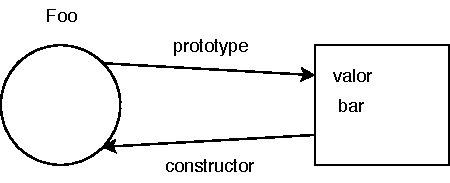
\includegraphics{Figures/Prototype}
\decoRule
\caption[\code{Foo}]{Diagrama del código y los objetos creados.}
\label{fig:prototype}
\end{figure}

Ahora que se mencionó este concepto, tiene sentido revelar que el constructor de clase \code{Object} no es otra cosa más que una función, y sus métodos \code{toString}, \code{valueOf}, ó \code{hasOwnProperty} forman parte de su "`prototipo"'. Ahora supongamos el siguiente código:

\begin{lstlisting}
var a = new Object();

console.log(a.toString());
\end{lstlisting}

La instancia \code{a} también tiene una propiedad del prototipo. Pero en este caso, en vez de ser \code{prototype}, la misma se llama \code{\_\_proto\_\_}. Una definición vaga sería que las funciones están vinculadas a un prototipo mediante su propiedad \code{prototype} mientras que las instancias se vinculan a su prototipo mediante la propiedad \code{\_\_proto\_\_}. La forma "`genérica"' definida en el estandar de ECMAScript cuando se habla del prototipo, es mediante el término \code{[[Prototype]]}.

Ahora, ?`qué sucede exactamente al momento de hacer \code{a.toString()}? En realidad lo que sucede es que se busca dentro del objeto de la instancia de \code{a} por una propiedad \code{toString}, pero al no encontrarse, se seguirá buscando en su \code{[[Prototype]]} (y en caso de no encontrarse, seguiría recursivamente hasta llegar a \code{null}). Ésto es lo que se denomina la cadena del prototipo ("`prototype chain"').

\begin{figure}[th]
\centering
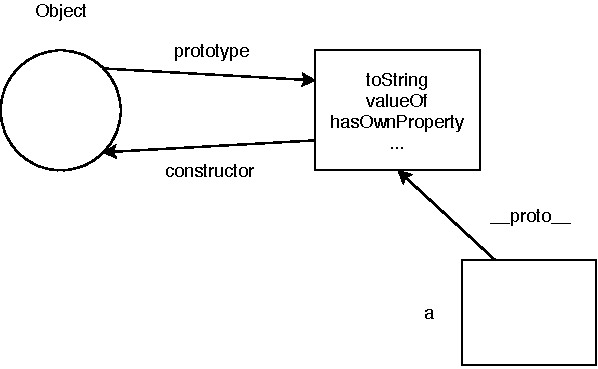
\includegraphics{Figures/Prototype2}
\decoRule
\caption[\code{Object}]{Diagrama del código y la instancia de \code{a}.}
\label{fig:prototype2}
\end{figure}

Sobre el uso del \code{prototype} se hablará con más detalle de esto en las secciones \ref{clases} y \ref{herencia}, donde en ésta última se hará mención a su rol en la herencia prototipada. % Introducción
% Chapter 2

\chapter{Sistema de Tipos} % Main chapter title

\label{Chapter2} % For referencing the chapter elsewhere, use \ref{Chapter1} 

%----------------------------------------------------------------------------------------

JavaScript es un lenguaje de "`scripting"', con tipado dinámico y un sistema de tipos débil. Generalmente, en este tipo de lenguajes interpretados no es necesario definir el tipo de una variable al momento de declararla, por lo que es lógico preguntarse ?`Es JavaScript un lenguaje seguro?.

%----------------------------------------------------------------------------------------

\section{Tipos primitivos}

Tal como se mencionó en el Capítulo \ref{Chapter1}, existen solamente 7 tipos primitivos del lenguaje:

\begin{itemize}
\item \code{undefined}
\item \code{null}
\item \code{number}
\item \code{string}
\item \code{boolean}
\item \code{symbol}
\item \code{object}
\end{itemize}

Algunos autores consideran que \code{Object} no es un tipo primitivo, sino que es un tipo que hereda de \code{Null}. Por otro lado, hay que mencionar que las funciones en JavaScript son consideradas objetos, por lo que \code{Function} es un subtipo de \code{Object}.

%----------------------------------------------------------------------------------------
 % Sistema de tipos
\chapter{Paradigma funcional}

\label{Chapter3}

% -----

Entre los puntos fuertes que posee el lenguaje, es indiscutible decir que las funciones son uno de los ejes principales. Sin embargo, ?`qué tan ligado está el lenguaje al paradigma de programación funcional?. ?`Soporta todas sus características?.

Es sabido que algunos conceptos como las funciones de alto orden están vinculadas con el paradigma funcional, mientras que también se conoce que JavaScript permite el pasaje de funciones como parámetros, o el retorno de las mismas como valores. En este capítulo se realizará un análisis sobre las mismas, para poder entender qué tan cerca o lejos está el lenguaje de las características del paradigma.

% -----

\section{Recursividad}

Al igual que los lenguajes sintáticamente similares a JavaScript, la recursión es una técnica que se aplica con naturaleza. Siempre que la función no sea anónima (es decir, que tenga un nombre), se puede aplicar recursión directa sin problemas. Además, el soporte para la recursión mutua también es posible gracias a la característica de \textit{hoisting}.

Cualquiera de las formas vistas en el Capítulo 1 son válidas para definir una función recursiva. A continuación se presentan ejemplos de las mismas, mostrando recursión directa y cruzada:

\begin{lstlisting}[title={Ejemplos de funciones recursivas}]
// Función recursiva con función como declaración
function sumatoria(n) {
  return n > 0 ? n + sumatoria(n - 1) : 0;
}

// Función recursiva con función como expresión
var factorial = function(n) {
  return n > 0 ? n * factorial(n - 1) : 1;
};

// Recursión cruzada
var esPar = num => (num === 0 ? true : esImpar(num - 1));
var esImpar = num => (num === 0 ? false : esPar(num - 1));
\end{lstlisting}

\section{Funciones puras}

Las funciones puras son otra de las claves del paradigma funcional. Esto es, funciones que bajo la misma entrada, siempre devuelven el mismo resultado. Los beneficios que trae el uso de las funciones puras, es la testeabilidad, predictibilidad, y la falta de efectos colaterales.

Por suerte, en el lenguaje se pueden escribir fácilmente funciones puras. Lamentablemente el lenguaje no posee ninguna directiva, y tampoco existe una herramienta concreta para determinar la pureza (o impureza) de una función, más que el conocimiento del programador.

A continuación, se mencionan algunas prácticas para evitar las funciones impuras:

\begin{itemize}
  \item Evitar el uso de variables que estén fuera del ámbito (scope) de la función. Esto incluye también a las variables globales del navegador.
  \item Evitar el uso del DOM o de variables del browser como \code{document} o \code{window}.
	\item Evitar el uso de \code{Math.random}, valores azarosos o cambiantes como el día y la hora actual.
	\item Evitar peticiones bajo el protocolo HTTP u otras que dependan del estado de la red.
	\item Evitar imprimir por pantalla o por consola, o cualquier mecanismo de I/O.
	\item Evitar la mutabilidad de datos. Recordar que los objetos en JS se manejan por referencia. Para éste ítem, se recomienda aplicar prácticas de inmutabilidad, o el uso de alguna librería externa.
\end{itemize}

\section{Funciones de primera clase y orden superior}

Una de las características más destacables del lenguaje es que las funciones son objetos, que a su vez se pueden almacenar como valores. Gracias a esto, resulta extremadamente simple el pasaje de funciones como argumentos, así como también devolver funciones como un valor de retorno.

\section{Evaluación ansiosa (estricta) y perezosa (no estricta)}

Uno de los puntos más cuestionables cuando se analiza a JavaScript dentro del paradigma funcional es la de la evaluación ansiosa y perezosa. % Programación funcional
\chapter{Paradigma orientado a objetos}

\label{Chapter4}

% -----

Uno de los debates principales sobre JavaScript es su soporte hacia el paradigma orientado a objetos.

% -----

\section{Clases}


Previo a la salida de ES6 (es decir, en la version 5 de JavaScript) la creación de clases en JavaScript se realiza mediante el uso de patrones para la creación de objetos. La realidad es que en JavaScript no existe un soporte formal o natural para las clases, sino que hay que recurrir a estos patrones para simularlo. Éstos son:

\begin{itemize}
	\item Factory
	\item Constructor
	\item Prototype
	\item Dynamic Prototype
\end{itemize}

\section{Herencia}

Como se ha mencionado anteriormente, JavaScript tiene la particularidad de tener la herencia prototipada en vez de la herencia clásica.



\section{Encapsulamiento}

\section{Polimorfismo}

\section{Abstracción}

\section{Modularidad}

\section{Principio de ocultación}

\section{Lo bueno, lo malo, lo feo...} % Programación orientada a objetos
%\chapter{Expresiones}

\label{Chapter5}

% ----

Intro capítulo

% ----

\section{\code{==} versus \code{===}}

\section{Coerción}

\section{Lo bueno, lo malo, lo feo...} % Expresiones
%\chapter{Expresiones}

\label{Chapter6}

% ----

Intro del capitulo

% ----

\section{\code{==} versus \code{===}}
 % Scope
%\chapter{\code{this} en JavaScript}

\label{Chapter6}

% ----

Intro del capitulo

% ----

\section{...}

\section{Lo bueno, lo malo, lo feo...} % this en JavaScript

%----------------------------------------------------------------------------------------
%	THESIS CONTENT - APPENDICES
%----------------------------------------------------------------------------------------

%\appendix % Cue to tell LaTeX that the following "chapters" are Appendices

% Include the appendices of the thesis as separate files from the Appendices folder
% Uncomment the lines as you write the Appendices

%% Appendix A

\chapter{Frequently Asked Questions} % Main appendix title

\label{AppendixA} % For referencing this appendix elsewhere, use \ref{AppendixA}

\section{How do I change the colors of links?}

The color of links can be changed to your liking using:

{\small\verb!\hypersetup{urlcolor=red}!}, or

{\small\verb!\hypersetup{citecolor=green}!}, or

{\small\verb!\hypersetup{allcolor=blue}!}.

\noindent If you want to completely hide the links, you can use:

{\small\verb!\hypersetup{allcolors=.}!}, or even better: 

{\small\verb!\hypersetup{hidelinks}!}.

\noindent If you want to have obvious links in the PDF but not the printed text, use:

{\small\verb!\hypersetup{colorlinks=false}!}.

%\include{Appendices/AppendixB}
%\include{Appendices/AppendixC}

%----------------------------------------------------------------------------------------
%	BIBLIOGRAPHY
%----------------------------------------------------------------------------------------

%\printbibliography[heading=bibintoc]

%----------------------------------------------------------------------------------------

\end{document}  
